\section{\lTechnique\ -- Learning in Space}
\label{sec:sampling}

In this paper, we explore an alternative approach to learning job runtime
properties online in order to facilitate cluster job scheduling.  The approach
is motivated by the following
%  \lTechnique, a novel learning technique with a very different
%  approach for learning runtime properties of distributed jobs. \lTechnique makes
key observations about distributed jobs running in shared clusters: (1) a
distributed job has a spatial dimension, \ie it typically consists of many
tasks; (2) all the tasks in the same phase of a job typically execute exactly
the same code with the same settings~\cite{googleClusterData2011-2Schema,
personalCommunication:MarkAstley}, and  differ in that they process different
chunks of similarly sized data. \commentaj{Also, if there is a need to run different types
of tasks with different resource requirements, they are executed as a separate
jobs~\cite{googleClusterData2019Schema}.}
Hence, it is likely that their runtime behavior
will be statistically similar.

The above observations suggest that if the scheduler first schedules a few
sampled tasks of a job to run till finish, it can use the observed runtime
properties of those tasks to accurately estimate those of the whole job. 
In a module design, such an online learning scheme can be decoupled from the
cluster scheduler.  In particular, upon a job arrival, the predictor first
schedules sampled tasks of the job, called {\em pilot tasks}, till their
completion, to learn the job runtime properties. The learned job properties are
then fed into the cluster job scheduler, which can employ different scheduling
polices to meet respective SLOs.  Effectively, the new scheme learns job
properties in the spatial dimension, \ie {\em learning in space}.  We denote
the new learning scheme  as \lTechnique.

% \lTechnique is a generic learning approach which can be used for estimating
%runtime properties of distributed jobs.
%  different schedulers can then use the estimated values to come up with a
%  schedule to meet the desired scheduling goals.
%the property of other tasks of the job.

Intuitively, by using the execution of pilot tasks to predict the properties of
other tasks, \lTechnique avoids the primary drawback of history-based learning
techniques, \ie relying on job properties to remain stationary over time.

\subsection{Learning in Time vs. Learning in Space}
\label{sec:comparison}

\begin{table}[tp]
%\vspace{-0.05in}
\caption{Comparison of learning in time and space of job runtime properties.}
\label{table:proscons}
\centering
{\small
\vspace{-0.1in}
\begin{tabular}{|c|c|c|c|c|c|}
\hline
                        & Applicability & Adapti- & Accuracy & Runtime \\
	                &               &         veness     &          & overhead\\
%\hline
\hline
	Time & Recurring jobs & No/Yes & Depends  & No\\
	%based& ing jobs  & &      &\\
\hline
	Space &New/Recurring jobs & Yes & Depends & Yes\\
	 %based &    &&&\\
\hline
%\vspace{-0.2in}
\end{tabular}
}
\vspace{-0.1in}
\end{table}

Learning in space introduces two new challenges:
%
(1) its estimation can be affected by the variations of task runtime
properties, \ie task skew;
%
(2) delaying scheduling the remaining tasks of a job till the completion of
sampled tasks may potentially hurt the job's completion time.

Table~\ref{table:proscons} summarizes the pros and cons of the two
learning approaches along four dimensions:

\begin{itemize}%[leftmargin=*]
\item {\bf Applicability:} As discussed in \S\ref{sec:back:existing}, most history-based
predictors cannot be used for jobs of a new category or for categories
for which jobs are rarely executed.  In contrast, learning in space
has no such limitation; it can be applied to any new job.
\item {\bf Adaptiveness to change:} Furthermore, history-based predictors assume
job runtime properties persist over time, which often does not hold, as discussed 
in \S\ref{sec:back:whatsWrong}. In contrast, learning in space does not have such 
limitation.
\item {\bf Accuracy:}
The accuracy of the two approaches are directly affected by
how the two approaches learn, \ie in space versus in time.
The accuracy of history-based approaches is affected by how stable
the job runtime properties persist over time, while that  of
sampling-based approach is affected by the variation of the task runtime properties,
\ie the level of task skew.
%  \questionaj{Should we add a briefly add here the intuitive argument as why
%  ampling will work in task runtime skew? Similar to the one we added for 
%  the coflow paper. I have written this in Appendix \S\ref{sec:appendixSkew}.}
%
\item {\bf Runtime overhead:} The history-based approach
has an inherent advantage of having very low to zero runtime
overhead. It performs offline analysis of historical data to generate
a prediction model.
\rm{Afterwards there is almost no overhead in
estimating runtime characteristics of newly arriving jobs. Variations
of history-based predictors that use runtime feedback to update the
prediction models may have some cost, but usually such systems are
optimized to have low runtime update overhead.}  In contrast,
sampling-based predictors do not have offline cost, but
need to first run a few pilot tasks till completion
before scheduling the remaining tasks. This may potentially
delay the job completion time.
%  Though, another point to be noted is that the
%  sampling based systems do not have any offline cost.
\end{itemize}

The above qualitative comparison of the two learning approaches raises the
following two questions:
(1) Can learning in space be more accurate than learning in time?
(2) Can {delaying scheduling} the remaining tasks of a job till the completion
of sampled tasks be more than compensated by the improved accuracy, so that the
overall job performance, \eg completion time, is improved?
%
We answer the first question via quantitative, trace and experimental analysis
in \S\ref{sec:accuracy} and the second question via a case study of cluster job
scheduling using the two types of predictors in \S\ref{sec:study}.


\if 0
\subsection{Design Issues}
\label{sec:sampling:designissues}

While making any design decision for implementing a \lTechnique based system
two things need to be considered. (1) What impact will it have on the
prediction accuracy?  (2) What impact will it have on scheduling efficiency?

The most important decision for any sampling based system is deciding the
number of tasks to be sampled. The number of samples affect both the prediction
accuracy and the efficiency as well. The other design decisions, primarily
impact either accuracy or efficiency.
%
%The key design decisions in implementing a \lTechnique based system can be
%grouped into following two broad categories (1) those have primary impact on
%prediction accuracy and (2) which are driven by cluster or scheduling constraints.

\subsection{How many tasks to sample?}
\label{sec:sampling:numpilots}
%The major thing to decide when learning using the \lTechnique is the number of
%sample tasks to be used.  Though, it is true that 
The accuracy of sampling will increase with the number of tasks sampled, we
show this in \S\ref{sec:comparison:quantity}. However, job properties can be
estimated, and in turn, the non-pilot tasks of the job can be scheduled,
only after the pilot tasks finish.  So, too many pilot tasks might delay the job
scheduling. Deciding the number of tasks to be sampled is a trade-off between,
accuracy and sampling delay. To avoid solving a dual-objective optimization
problem, we propose a simple heuristic to untangle the dual objectives.
Specifically, we first study how the number of samples affects the sampling
accuracy. Then, look for a sweet spot, \ie the smallest
number of samples that brings the most improvement in prediction accuracy. 

%Many other factors like oversubscription ratio of
%the cluster, accuracy need of the scheduling system can influence the decision.
%We elaborate more on this in
%\S\ref{sec:comparison}. 
%
%If all the jobs are fairly similar in width (total number of tasks) the obvious
%choice is using a constant number of pilot tasks. However, if jobs are of
%varying width, the natural choice is to use a fixed fraction of the total
%number of tasks in the job.
%
In our case-study \S\ref{sec:study} we found using ~5\% of the total number of
tasks as pilot task works best for that design \S\ref{sec:sim:numPilots}.

\subsection{Scheduling the pilot tasks and estimating job properties}
Once we have decided the number of pilot tasks. Next step is to
efficiently schedule them and upon their completion estimate the desired
job properties.
%using values measured by executing sampling tasks. 
This work can be understood in following four major steps. 

\paragraph{How to choose pilot tasks?} \\ 
Now when we know the number of pilot tasks for a job next step is to identify
the specific tasks to be sampled. The simplest way is to randomly pick sampling
tasks.  However, in many cases it might be desirable to finish sampling as fast
as possible. In such cases we want to meet the following two conditions (1)
Pilot tasks of the same job are not contending for runtime resources among
themselves. (2) Assign the least busy resources to sampling tasks. 
%As this will elongate the process of sampling. Also, in general, to
%speed up the process of sampling it will be preferable 
The above conditions might influence which tasks to be
picked as sampling task. 

Additionally, there might be certain system specific conditions which can
influence this decision. For instance, if for a framework, tasks arrive in
waves and there might not be enough tasks in the first wave to provide many
options to choose sampling tasks. In such scenarios scheduler might default to
FIFO for assigning pilot tasks.

In our case-study \S\ref{sec:study} we select sampling tasks in FIFO order.  We
discuss the reason behind our decision in detail in
\S\ref{sec:design:namepredict}.

\paragraph{In what order to schedule pilot tasks?} \\
Once we have identified sampling task, the next challenge is to determine their
scheduling order . It might not be the case that we always have enough resource
to schedule all the sampling tasks of a job in parallel. Sampling tasks of
different jobs also might compete with each other. How to resolve this
conflict?. Such decisions need to be made depending upon the constraints and
the needs of the specific case.

\paragraph{Should we skip sampling for some jobs?} \\
In general, in a sampling based system, all the other tasks of a job are not
scheduled until the pilot tasks finish (if no other task is waiting to be
scheduled and resources are available then for work conservation non-sampling
tasks can be scheduled in parallel to sampling tasks). However, such a design
choice can inadvertently lead to higher Jots for some jobs, particularly for
thin jobs, \eg a two-task job would end up serializing scheduling its two
tasks, one for the sampling purpose.

To avoid JCT degradations for thin jobs, sampling could be avoided for them.
However, in systems where bloating of JCT is not a concern, even thin jobs can
go through sampling.

%In our case-study \S\ref{sec:study} we skip sampling for jobs with less than 30
%tasks.  We discuss this in \S\ref{sec:study:design} and provide a sensitivity
%analysis for varying thinlimit in \S\ref{sec:sim:sa}.
\paragraph{What to do after sampling?} \\
Once the sampling is over, different statistical mechanisms could be deployed
to estimate job properties.  One could either calculate point estimates like
mean, median or can use the distribution based techniques like
bootstrapping or techniques similar to the one described in 3Sigma \cite{3Sigma}.

\fi



\if 0
\begin{figure*} 
\centering
\subfigure[\vspace{-0.2in}Google trace -- application name -- average task runtime]
{
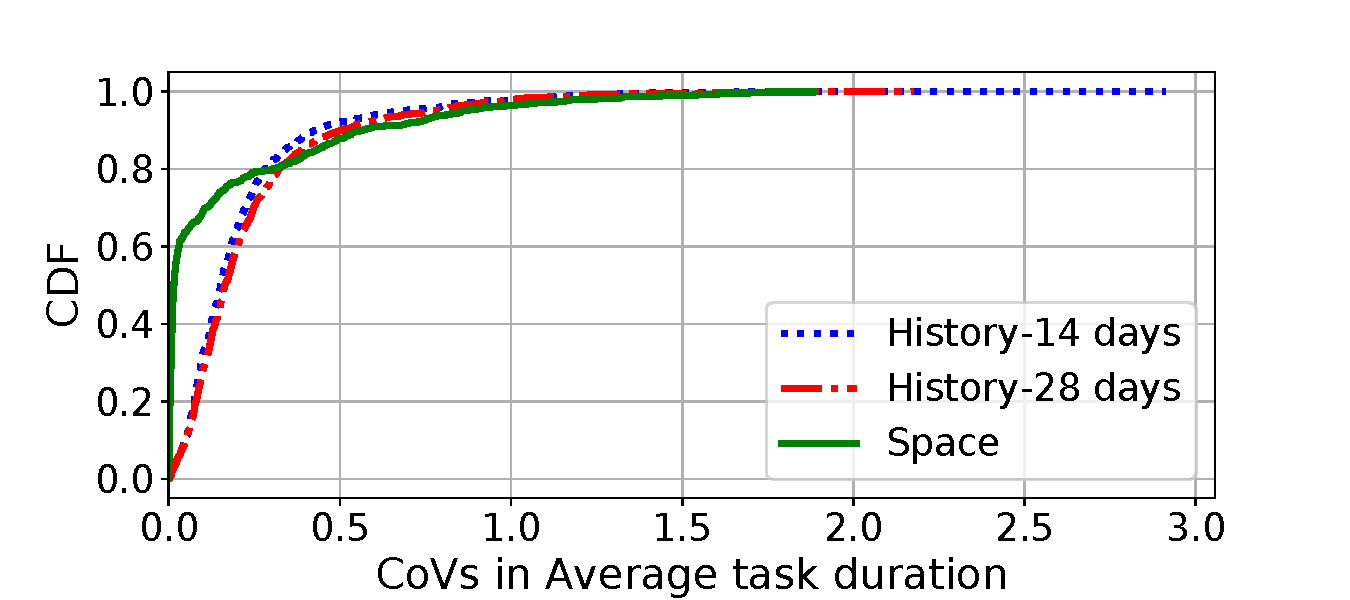
\includegraphics[width=0.48\linewidth]{figures/trace_analysis/slidingWindow_analysis_cdf_of_covs_in_avg_task_dur_for_application_name_in_google11_judgement_day_28.pdf}	% done
%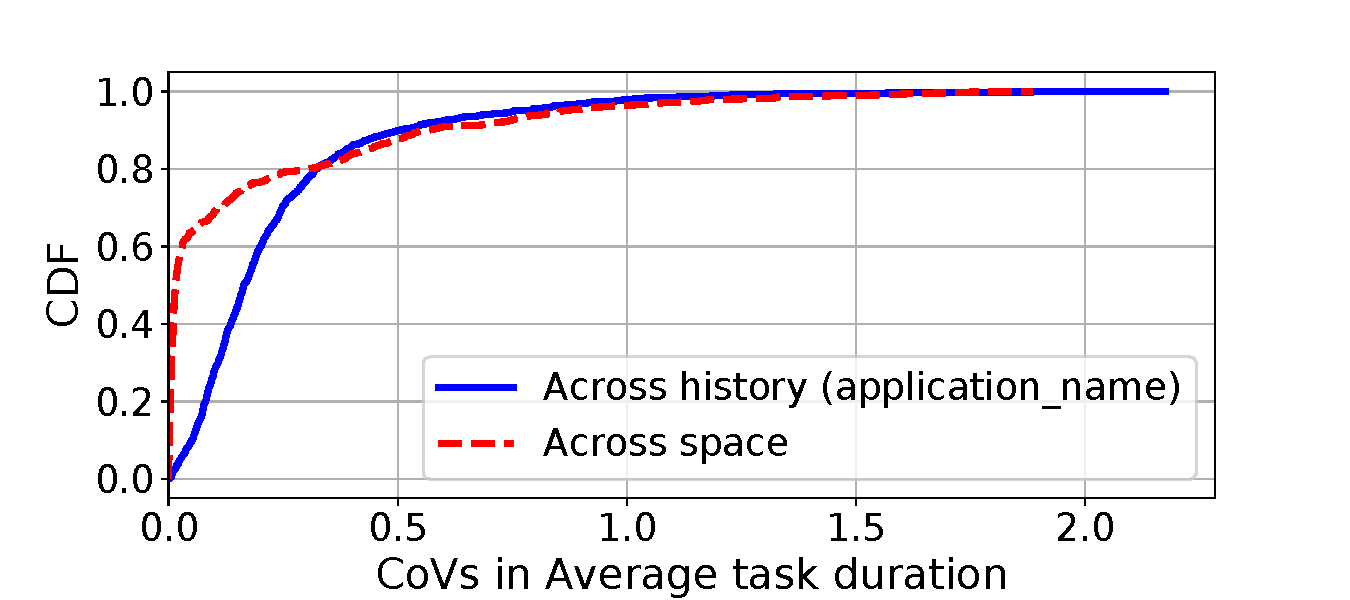
\includegraphics[width=0.48\linewidth]{figures/trace_analysis/slidingWindow_analysis_cdf_of_covs_in_avg_task_dur_for_application_name_in_google11Trace_first_day_0_window_period_28.pdf}	% done
\label{fig:trace_analysis:google11:task_dur}
}
\subfigure[\vspace{-0.2in}Google trace -- application name -- mean CPU usage]
{
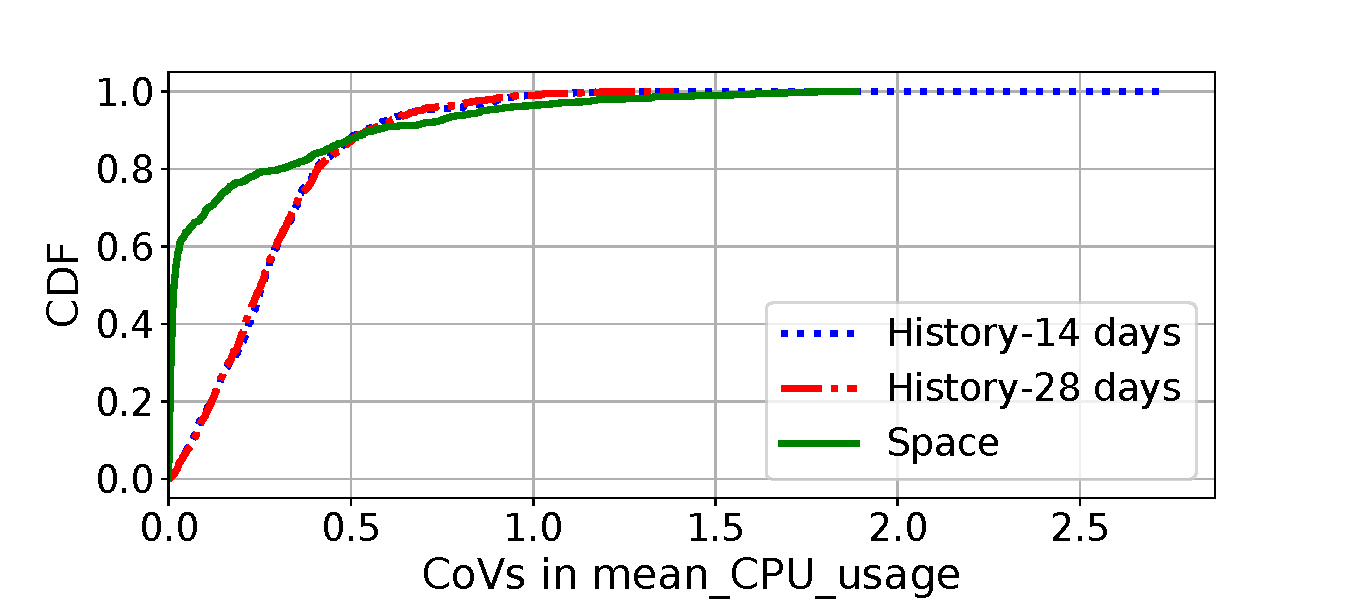
\includegraphics[width=0.48\linewidth]{figures/trace_analysis/slidingWindow_analysis_cdf_of_covs_in_mean_CPU_usage_for_application_name_in_google11_judgement_day_28.pdf}	% done
%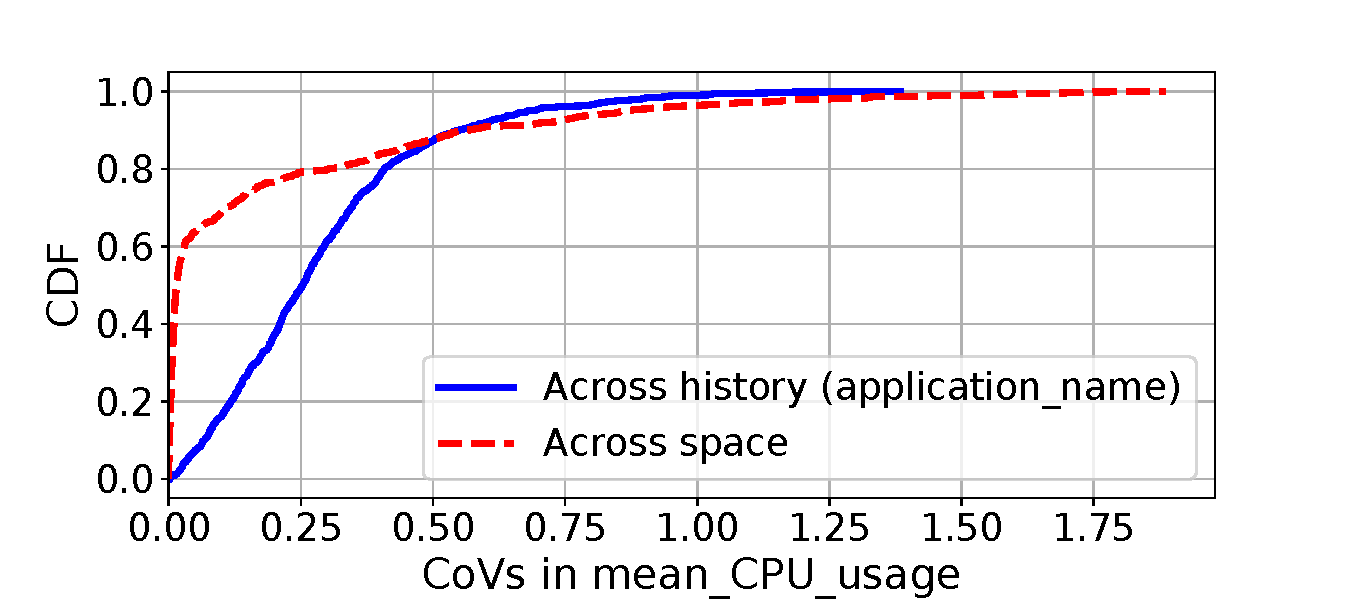
\includegraphics[width=0.48\linewidth]{figures/trace_analysis/slidingWindow_analysis_cdf_of_covs_in_mean_CPU_usage_for_application_name_in_google11Trace_first_day_0_window_period_28.pdf}	% done
\label{fig:trace_analysis:google11:cpuUsage}
}
\subfigure[\vspace{-0.2in}Google trace -- application name -- mean disk IO time]
{
%\vspace{-0.2in}
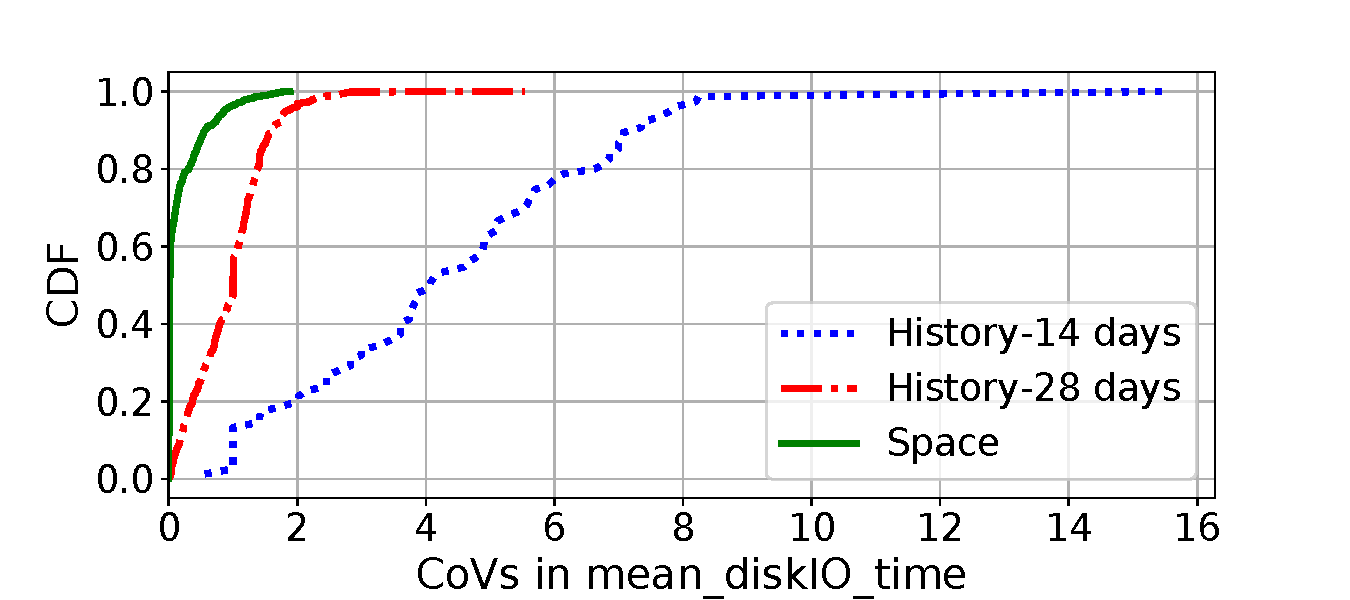
\includegraphics[width=0.48\linewidth]{figures/trace_analysis/slidingWindow_analysis_cdf_of_covs_in_mean_diskIO_time_for_application_name_in_google11_judgement_day_28.pdf}	% done
%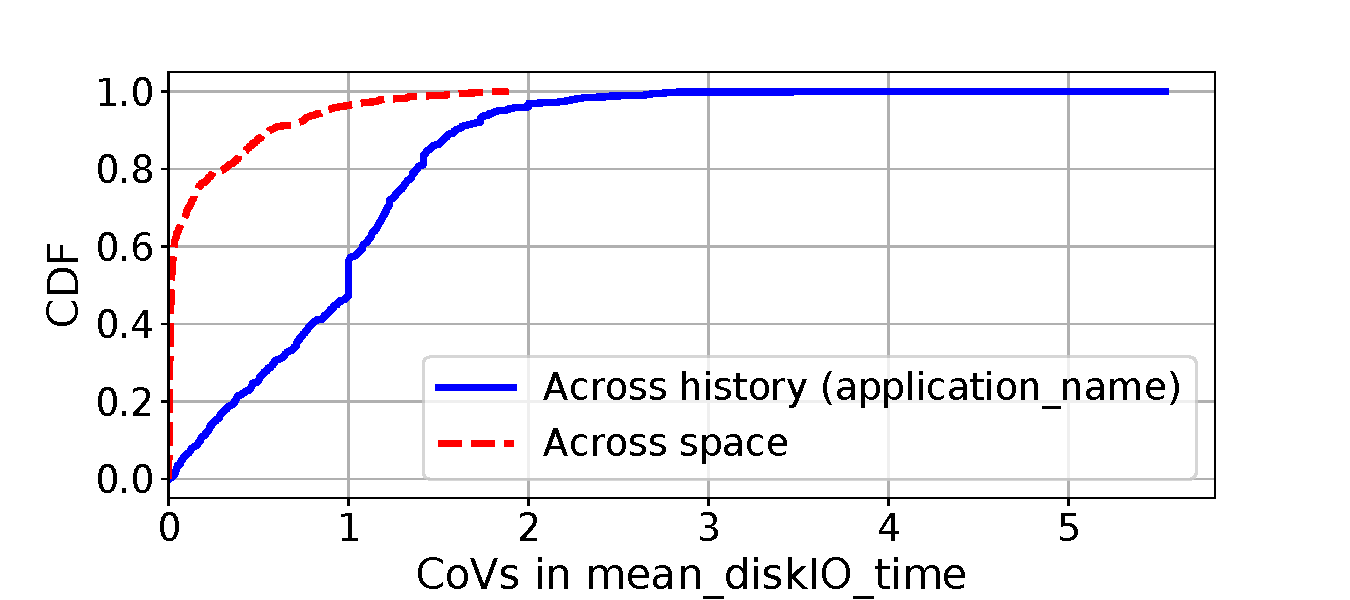
\includegraphics[width=0.48\linewidth]{figures/trace_analysis/slidingWindow_analysis_cdf_of_covs_in_mean_diskIO_time_for_application_name_in_google11Trace_first_day_0_window_period_28.pdf}	% done
\label{fig:trace_analysis:google11:diskIO}
}
\subfigure[\vspace{-0.2in}2Sigma trace -- user name -- average task runtime]
{
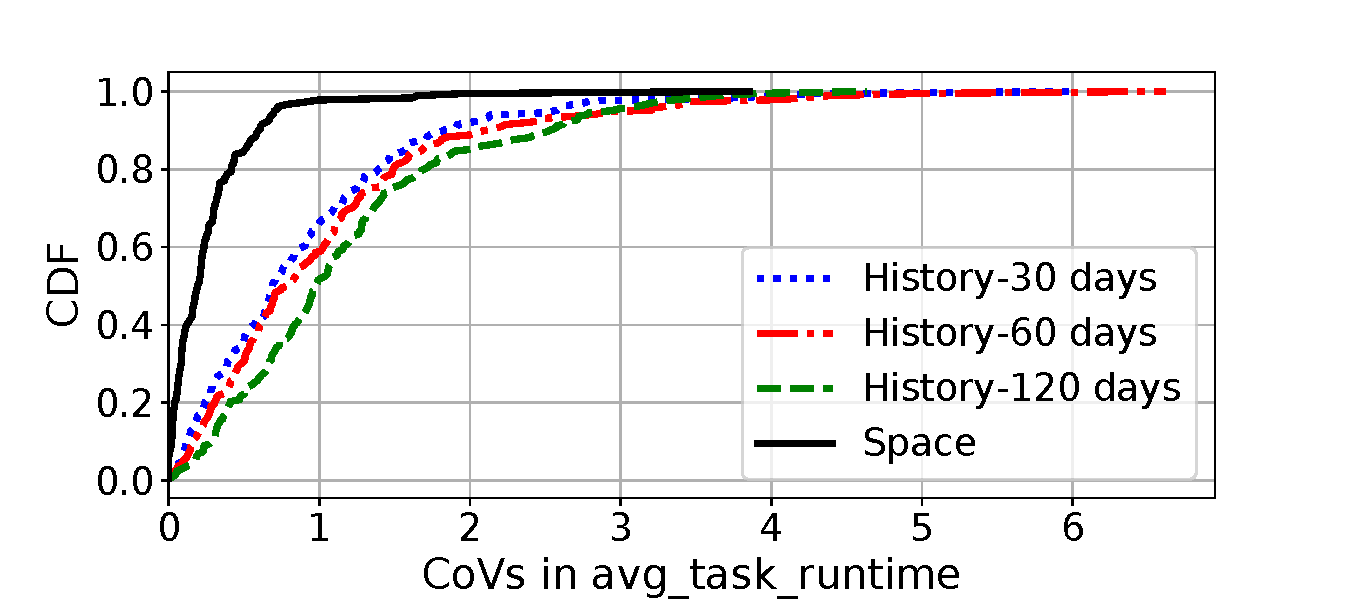
\includegraphics[width=0.48\linewidth]{figures/trace_analysis/slidingWindow_analysis_cdf_of_covs_in_avg_task_runtime_for_user_name_in_2Sigma_judgement_day_227.pdf}	% done
%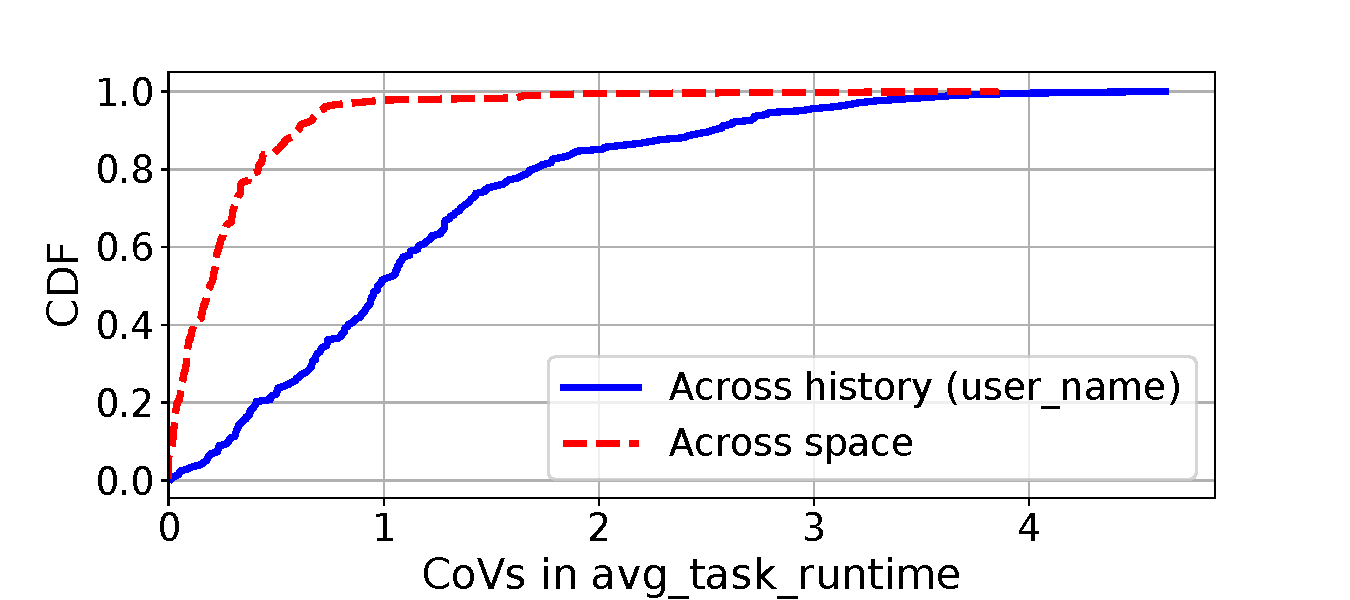
\includegraphics[width=0.48\linewidth]{figures/trace_analysis/slidingWindow_analysis_cdf_of_covs_in_avg_task_runtime_for_user_name_in_2SigmaTrace_first_day_107_window_period_120.pdf}	% done
\label{fig:trace_analysis:2Sigma:task_dur}
}
\caption{Trace Analysis. 
Solid curves show CDF of coefficients of variation ($\frac{\sigma}{\mu}$) in
average task runtime, task CPU usage and time spent by tasks in disk IO
for all jobs in the 28 (120) day period for the Google (2Sigma) trace
having same feature value. Dashed curves in the corresponding figures
shows CDF of CoVs across tasks of a job for the corresponding properties, for all jobs on
29th (121st) day.
}
\vspace{-0.1in}
\label{fig:trace_analysis}
\end{figure*}
\fi
